\chapter{TCP超时与重传}
\minitoc

\section{引言}
到目前为止,我们并没有过多地涉及效率与性能,而主要关注操作的正确性。在本章及接下来的两章中,我们不仅讨论 TCP执行的基本任务,还关心其执行效率。由于下层网络
层(IP)可能出现丢失、重复或失序包的情况,TCP 协议提供可靠数据传输服务。为保证数据传输的正确性,TCP重传其认为已丢失的包。TCP根据按收端返回至发送端的一系列确认
信息来判断是否出现丢包。当数据段或确认信息丢失,TCP启动重传操作,重传尚未确认的数据。TCP拥有两套独立机制来完成重传,一是\textbf{基于时间},二是\textbf{基于确认信息的构成}。第二
种方法通常比第一种更高效。

TCP 在发送数据时会设置一个计时器,若至计时器超时仍未收到数据确认信息,则会引发相应的超时或基于计时器的重传操作,计时器超时称为重传超时(RTO)。另一种方式的重
传称为快速重传,通常发生在没有延时的情况下。若 TCP 累积确认无法返回新的ACK,或者当ACK 包含的选择确认信息(SACK)表明出现失序报文段时,快速重传会推断出现丢
包。通常来说,当发送端认为接收端可能出现数据丢失时,需要决定发送新(未发送过的)数据还是重传。本章内容将详细讨论 TCP怎样判断出现报文段丢失及其响应操作。发送数
据量问题,即由丢包而引发的拥塞控制机制,将会在第16章具体介绍。这里,我们探讨如何根据某个连接的 RTT来设置 RTO,基于计时器的重传机制,以及TCP快速重传操作。另
外我们也会看到SACK 怎样帮助确定丢失数据、失序和重复IP 包对TCP 行为的影响,以及TCP重传时改变包大小的方法。最后我们简要讨论一些可能导致TCP 出现过分积极或被动
行为的攻击方法。

\section{简单的超时与重传举例}
我们已经看到一些超时和重传的例子。
\begin{tcolorbox}
    \begin{enumerate}
        \item 在第8章ICMP 目的不可达(端口不可达)的例子中,采用UDP 的TFTP 客户端使用简单(且低效)的超时和重传策略:设置足够大的超时间隔,每5秒进行一次重传。
        \item 第13章的尝试与不存在的主机建立连接中,我们看到TCP 在尝试建立连接的过程中,在每次重传时采用比上次更大的延时间隔。
        \item 在第3章的以太网冲突中,我们也可以看到相关操作。
    \end{enumerate}
\end{tcolorbox}

上述机制都是由计时器超时引发的。

我们首先来看 TCP的基于计时器的重传策略。先建立一个连接,并发送一些数据验证连接正常。然后断开连接的一端,这时再发送一些数据,观察 TCP 的操作。这里我们采用
Wireshark 来跟踪记录连接状况(见图14-1)。

\begin{figure}[!htb]
	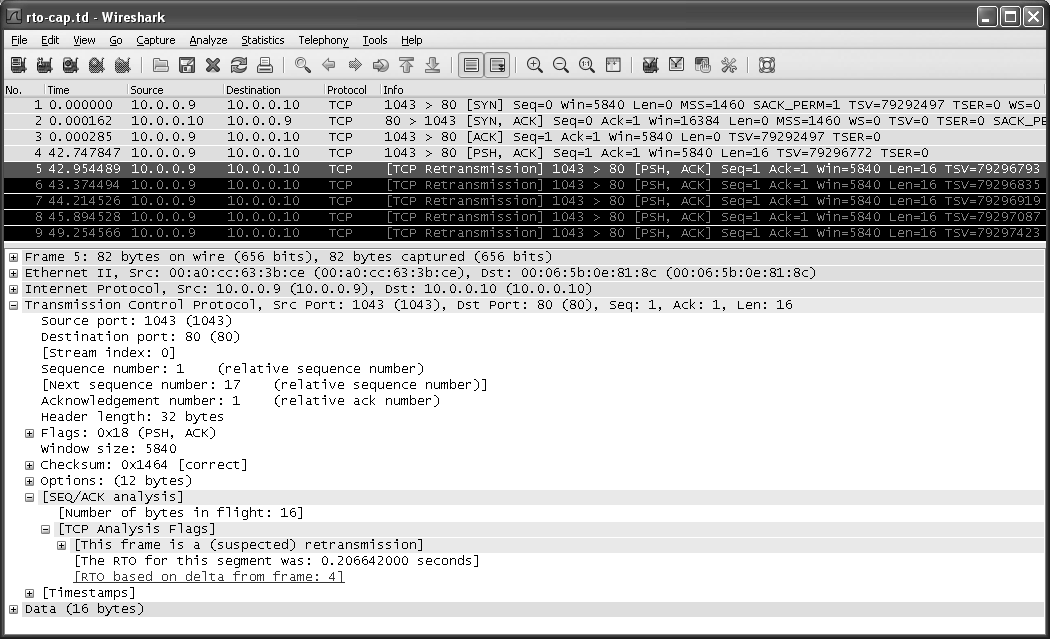
\includegraphics[width=1.0\textwidth]{imgs/14/14-1.png}
	\caption{tcp重传简单的例子}
\end{figure}

报文段1、2、3为TCP建立连接的握手过程。连接建立完成后,Web 服务器处于等待 Web 请求的状态。在发出请求前,我们先断开服务器端主机的连接。在客户端输入如下命令:
\begin{verbatim}
    Linux% telnet 10.0.0.10 80
    Trying 10.0.0.10...
    Connected to 10.0.0.10.
    Escape character is '^]'.
    GET / HTTP /1.0
    Connection closed by foreign host.
\end{verbatim}

该请求无法传输至服务器端,因此它会在客户端的TCP 队列中存储一段时间。此时采用 netstat 命令读取客户端队列状态显示为非空:

\begin{verbatim}
Active Internet connections (w/o servers)
Proto Recv-Q Send-Q     Local Address       Foreign Address     State
tcp        0     18     10.0.0.9:1043       10.0.0.10:www       ESTABLISHED
\end{verbatim}

可以看到发送队列中有18字节的数据,等待被传送至Web 服务器。这18个字节包含了之前显示的请求命令以及回车换行。其他的输出细节(包括地址和状态信息)会在下面涉及。

报文段4为客户端首次尝试发送 Web 请求,时间为 42.748s。0.206s 以后,在42.9545发送了第二次请求。接着在 43.374S,即 0.420s后,再次尝试请求。后续的请求(重传)时刻
分别为 44.215、45.895以及 49.255s,间隔分别为1.680和 3.360s。

每次重传间隔时间加倍称为\textcolor{red}{二进制指数退避}(binary exponential backoff),我们在第13章的TCP 尝试建立连接失败时提到过,后面将会详细讨论。自首次请求至连接完全失效,
总时间为15.5min。随后,客户端会显示如下错误信息:
\begin{verbatim}
    Connection closed by foreign host.
\end{verbatim}

逻辑上讲,TCP 拥有两个阈值来决定如何重传同一个报文段。主机需求 RFC[RFC1122]描述了这两个阈值,在第13 章中也提到过。R1表示 TCP 在向IP 层传递“消极建议”(如重新
评估当前的I路径)前,愿意尝试重传的次数(或等待时间)。R2(大于R1)指示 TCP 应放弃当前连接的时机。R1 和R2应分别至少设为三次重传和100秒。对连接的建立过程(发送
SYN 报文段),阈值设置与数据段传输有所区别,针对SYN报文段的R2应最少设为3分钟。

Linux 系统中,对一般数据段来说,R1 和 R2的值可以通过应用程序,或使用系统配置变量 \verb|net.ipv4.tcp_retries1| 和 \verb|net.ipv4.tcp_retries2|设置。变量值为重传次数,而不是以时间为
单位。\verb|tcp_retries2|默认值为15,对应约为\(13-30\)分钟,根据具体连接的 RTO而定。\verb|net.ipv4.tcp_retries1| 默认值为3。对于SYN报文段,变量 \verb|net.ipv4.tcp_syn_retries|
和 \verb|net.ipv4.tcp_synack_retries| 限定重传次数,默认值为5(约180秒)。Windows 也有相应控制 TCP行为的变量,包括R1 和 R2。通过下列注册表项可以修改对应值 [WINREG]:

\begin{verbatim}
    HKLM\System\CurrentControlSet\Services\Tcpip\Parameters
    HKLM\System\CurrentControlSet\Services\Tcpip6\Parameters
\end{verbatim}

最主要的值为 TepMaxDataRetransmissions,对应 Linux 中的 \verb|tcp_retries2| 变量,其默认值为5。至此我们看到,TCP 需要为重传计时器设置超时值,指示发送数据后等待ACK的
时间。假设 TCP 只工作在静态环境中,那么很容易为超时设置一个合适的值。由于 TCP 需要适应不同环境进行操作,可能随着时间不断变化,因此需基于当前状态设定超时值。例
如,若某个网络连接失败,需重新建立,RTT也会随之改变(可能变化很大)。也就是说,TCP 需要动态设置 RTO(重传超时)。下面我们讨论这一问题。

\section{设置重传超时}
TCP 超时和重传的基础是怎样根据给定连接的 RTT设置 RTO。若TCP 先于 RTT 开始重传,可能会在网络中引入不必要的重复数据。反之,若延迟至远大于 RTT 的间隔发送重
传数据,整体网络利用率(及单个连接吞吐量)会随之下降。由于 RTT的测量较为复杂,根据路由与网络资源的不同,它会随时间而改变。TCP 必须跟踪这些变化并适时做出调整来维
持好的性能。

TCP 在收到数据后会返回确认信息,因此可在该信息中携带一个字节的数据(采用一个特殊序列号)来测量传输该确认信息所需的时间。每个此类的测量结果称为 RTT 样本(RTT
sample)。TCP 首先需要根据一段时间内的样本值建立好的估计值。第二步是怎样基于估计值设置 RTO。RTO 设置得当是保证TCP 性能的关键。

每个TCP连接的 RTT均独立估算,并且重传计时器会对任何占用序列号的在传数据(包括SYN 和FIN报文段)计时。如何恰当设置计时器一直以来都是研究的热点问题,近年
来也取得了一些成果。本章节将探讨计算 RTO 计算方法在演进历程中的一些重要里程碑。首先我们介绍第一个(“经典”)方法,详见[RFCO793]。

\subsection{经典方法}
最初的 TCP 规范 [\href{https://datatracker.ietf.org/doc/html/rfc0793#section-3.7}{RFC0793}]采用如下公式计算得到平滑的 RTT 估计值(称为 SRTT):
\begin{equation}
    SRTT = \alpha(SRTT) + (1 - \alpha) RTT,
\end{equation}

这里,SRTT 是基于现存值和新的样本值 RTT.得到更新结果的。常量a为平滑因子,推荐值0.8~0.9。每当得到新的样本值,SRTT 就会做出相应的更新。从a的设定值可以看
到,新的估计值有80\% ~90\%来自现存值,10\% ~20\%来自新测量值。这种估算方法称为指数加权移动平均(Exponentially Weighted Moving Average, EWMA)或低通过滤器 (low-
pass filter)。该方法实现起来较为简单,只要保存SRTT 的先前值即可得到新的估计值。

考虑到 SRTT 估计器得到的估计值会随 RTT 而变化,[\href{https://datatracker.ietf.org/doc/html/rfc0793#section-3.7}{RFC0793}] 推荐根据如下公式设置RTO:
\begin{equation}
    RTO = min(ubound, max(lbound, (SRTT)B))
\end{equation}

这里的B为时延离散因子,推荐值为1.3~2.0。ubound为RTO 的上边界(可设定建议值,如1分钟),lbound为 RTO 的下边界(可设定建议值,如1秒)。我们称该方法为经典方法,
它使得 RTO 的值设置为1秒,或约两倍的SRTT。对于相对稳定的RTT分布来说,这种方法能取得不错的性能。然而,若 TCP运行于 RTT 变化较大的网络中,则无法获得期望的效果。

\subsection{标准方法}
在[88]中,Jacobson 进一步分析了上述经典方法,即按照[RFC0793]设置计时器无法适应 RTT 的大规模变动(特别是,当实际的 RTT远大于估计值时,会导致不必要的重传)。
增大的RTT 样本值表明网络已出现过载,此时不必要的重传无疑会进一步加重网络负担。

为解决上述问题,可对原方法做出改进以适应RTT变动较大的情况。可通过记录 RTT测量值的变化情况以及均值来得到较为准确的估计值。基于均值和估计值的变化来设置
RTO,将比仅使用均值的常数倍来计算 RTO更能适应 RTT 变化幅度较大的情况。

[88] 中的图5和图6显示了采用[RFC0793]与同时考虑 RTT变化值的方法计算 RTO的对比情况。如果我们将 TCP 得到的 RTT测量样本值考虑为一个统计过程,那么同时测量
均值和方差(或标准差)能更好地估计将来值。对 RTT的可能值范围做出好的预测可以帮助TCP 设定一个能适应大多数情况的 RTO值。

正如 Jacobson 所述,平均偏差(mean deviation)是对标准差的一种好的逼近,但计算起来却更容易、更快捷。计算标准差需要对方差进行平方根运算,对于快速 TCP 实现来说代
价较大。(但这并非全部原因,可参见[G04] 中所述的有趣的“争论”历史。)因此我们需要结合平均值和平均偏差来进行估算。可对每个 RTT 测量值 M(前面称为 RTT.)采用如下算式:

\begin{equation}
    srtt \leftarrow (1-g)(srtt) + (g)M
\end{equation}
\begin{equation}
    rttvar \leftarrow (1-h)(rttvar) + (h)(|M-srtt|)    
\end{equation}
\begin{equation}
    Rto = srtt + 4(rttvar)
\end{equation}

这里,srt 值替代了之前的SRTT,且rttvar 为平均偏差的EWMA,而非采用先前的B来设置 RTO。这组等式也可以写成另一种形式,对计算机实现来说操作较为方便:
\begin{equation}
    Err = M - srtt
\end{equation}
\begin{equation}
    srtt \leftarrow srtt + g(Err)
\end{equation}
\begin{equation}
    rttvar \leftarrow rttvar + h(|Err| - rttvar)
\end{equation}
\begin{equation}
    RTO = srtt + 4(rttvar)
\end{equation}

如前所述,srtt 为均值的EWMA,rttvar 为绝对误差IBrrl的EWMA。Err 为测量值 M与当前 RTT 估计值 srtt之间的偏差。srtt与 rttvar 均用于计算 RTO 且随时间变化。增量g为新
RTT 样本M占 srtt估计值的权重,取为1/8。增量h为新平均偏差样本(新样本M与当前平均值 srtt 之间的绝对误差)占偏差估计值 rttvar 的权重,取为1/4。当RTT变化时,偏差的增
量越大,RTO增长越快。8和及的值取为2的(负的)多少次方,使得整个计算过程较为简单,对计算机来说只要采用定点整型数的移位和加法操作即可,而无须复杂的乘除法运算。

\begin{tcolorbox}
    标准差公式:
    \begin{equation}
        \sigma = \sqrt\frac{\sum{(X-\mu)^2}}{N}
    \end{equation}
\end{tcolorbox}
比较经典方法与 Jacobson 的计算方法,平均 RTT 的计算过程类似(a等于1减增量g),只是采用的增量不同。另外,Jacobson 同时基于平滑 RTT 和平滑偏差计算RTO,而经典方
法简单采用平滑 RTT 的倍数。这是迄今为止许多 TCP 实现计算 RTO 的方法,并且由于其作为[RFC6298] 的基础,我们称其为标准方法,尽管在[RFC6298]中有一些改进。下面我们就
讨论这个问题。

\subsubsection{时钟粒度与 RTO 边界}

在测量 RTT的过程中,TCP 时钟始终处于运转状态。对初始序列号来说,实际TCP连接的时钟并非从零开始计时,也没有绝对精确的精度。相反地,TCP 时钟通常某个变量,
该变量值随着系统时钟而做出更新,但并非一对一地同步更新。TCP 时钟一个“滴答”的时间长度称为粒度。通常,该值相对较大(约500ms),但近期实现的时钟使用更细的粒度(如
Linux 采用1ms)。

粒度会影响 RTT的测量以及 RTO的设置。在[RFC6298]中,粒度用于优化 RTO 的更新情况,并给RTO设置了一个下界。计算公式如下!

这里的G为计时器粒度,1000ms 为整个 RTO 的下界值([RFC6298] 的规则(2.4)建议值)。因此,RTO 至少为1s,同时提供了可选上界值,假设为60s。

\subsubsection{初始值}

我们已经看到估计器怎样随时间进行更新,但同时也需要了解怎样设置初始值。在首个SYN 交换前,TCP 无法设置 RTO 初始值。除非系统提供(有些系统在转发表中级存了该信
息,见14.9节),否则也无法设置估计器的初始值。根据[RFC6298],RTO 的初始值为1s,而初始 SYN 报文段采用的超时间隔为3s。当接收到首个 RTT 测量结果M,估计器按如下方
法进行初始化:

\begin{equation}
    srtt +- M
    rttvar ‹- M/2
\end{equation}

我们已经了解了估计器的初始化和运行过程。RTO 的设置看似取决于得到的RTT采样值,下面我们将看到一些例外情况。
\subsubsection{重传二义性与Karn 算法}

在测量 RTT样本的过程中若出现重传,就可能导致某些问题。假这一个包的传输出现超时,该数据包会被重传,接着收到一个确认信息。那么该信息是对第一次还是第二次传输
的确认就存在二义性。这就是重传二义性的一个例子。

[KP87]指出,当出现超时重传时,接收到重传数据的确认信息时不能更新 RTT 估计值。这是 Kar 算法的“第一部分”。它通过排除二义性数据来解决 RTT估算中出现的二义性问
题。[RFC6298] 做出了相关要求。

假如我们在设置 RTO 过程中简单地将重传问题完全忽略,就可能将网络提供的一些有用信息也同时忽略(即网络中可能出现某些因素影响传输速度)。这种情况下,在网络不
再出现丢包前降低重传率有助于减轻网络负担。这也是下面指数退避行为的理论基础,见图14-1。

TCP 在计算 RTO 过程中采用一个退避系数(backoff factor),每当重传计时器出现超时,退避系数加倍,该过程一直持续至接收到非重传数据。此时,退避系数重新设为1(即二进
制指数退避取消),重传计时器返回正常值。对重传过程退避系数加倍,这是Kar 算法的“第二部分”。注意若 TCP 超时,同时会引发拥塞控制机制,以此改变发送速率(拥塞控制
将在第16 章详细讨论)。因此,Kam 算法实际上由两部分组成,如[KP89]所述:

当接收到重复传输(即至少重传一次)数据的确认信息时,不进行该数据包的RTT测量,可以避免重传二义性问题。另外,对该数据之后的包采取退避策略。仅
当接收到未经重传的数据时,该 SRTT 才用于计算 RTO。

Kam 算法一直作为 TCP 实现中的必要方法(自『RFC1122]起),然而也有例外情况。在使用 TCP 时间戳选项(见第13章)的情况下,可以避免二义性问题,因此Karn 算法的第-
部分不适用。

\subsubsection{带时间戳选项的 RTT测量}

TCP 时间戳选项(TSOPT)作PAWS算法的基础(第13章中已经提过),还可用作RTT 测量(RTTM)[RFC1323]。TSOPT 的基本格式第13 章中已经介绍过。它允许发送者在
返回的对应确认信息中携带一个32比特的数。

时间戳值(TSV)携带于初始SYN的 TSOPT 中,并在 SYN +ACK 的 TSOPT的 TSER部分返回,以此设定srtt、rttvar 与 RTO 的初始值。由于初始SYN 可看作数据(即同样采取
丢失重传策略且占用一个序列号),应测量其 RTT值。其他报文段中也包含 ISOPT,因此可结合其他样本值估算该连接的RTT。该过程看似简单但实际存在很多不确定因素,因为TCP
并非对其接收到的每个报文段都返回 ACK。例如,当传输大批量数据时,TCP 通常采取每两个报文段返回一个 ACK 的方法(见第15章)。另外,当数据出现丢失、失序或重传成功
时,TCP 的累积确认机制表明报文段与其 ACK之间并非严格的一一对应关系。为解决这些问题,使用时间戳选项的 TCP(大部分的 Linux 和 Windows 版本都包含)采用如下算法来测
量 RTT样本值:
\begin{enumerate}
    \item TCP 发送端在其发送的每个报文段的 TSOPT的TSV 部分携带一个32比特的时间戳值。该值包含数据发送时刻的 TCP 时钟值。
    \item 接收端记录接收到的 TSV 值(名为 TsRecent 的变量)并在对应的ACK 中返回,并且记录其上一个发送的 ACK 号(名 LastACK的变量)。回忆一下,ACK 号代表接收端(即ACK 的发送方)期望接收的下一个有序序号。
    \item 当一个新的报文段到达时,如果其序列号与LastACK 的值吻合(即为下一个期望接收的报文段),则将其 TSV 值存人 TsRecent。
    \item 接收端发送的任何一个 ACK 都包含 TSOPT,TsRecent 变量包含的时间戳值被写人其TSER部分。
    \item 发送端接收到 ACK 后,将当前 TCP 时钟减去 TSER 值,得到的差即为新的RTT样本估计值。
\end{enumerate}
FreeBSD、Linux 以及近期的Windows版本都默认启用时间戳选项。在Linux 中,系统配置变量 \verb|net.ipv4.top_timestamps|控制是否使用该选项(0代表禁用,1代表使用)。在
Windows 中,通过前面提到的注册表区域的 Tep13230pts 值来控制其使用。若值0,时间戳被禁用;若值为2,则启用。该键值没有设默认值(它并非默认存在于注册表中)。但若在
连接初始化过程中,TCP通信的另一方使用时间戳,则默认启用。

\subsection{Linux 采用的方法}

Linux 的RTT 测量过程与标准方法有所差别。它采用的时钟粒度为1ms,与其他实现方法相比,其粒度更细,TSOPT也是如此。采用更频繁的 RTT 测量与更细的时钟粒度,RTT测
量也更为精确,但也易于导致 rttvar 值随时间减为最小[LS00]。这是由于当累积了大量的平均偏差样本时,这些样本之间易产生相互抵消的效果。这是其 RTO 设置区别于标准方法的一
个原因。另外,当某个 RTT样本显著低于现有的 RTT估计值 srtt 时,标准方法会增大 rttvar。

为更好地理解第二个问题,首先回顾一下 RTO通常设置为 srtt +4(rttvar)。因此,无论最大 RTT 样本值是大于还是小于 srtt,rttvar 的任何大的变动都会导致 RTO增大。这与直觉
相反——若实际 RTT 大幅降低,RTO并不会因此增大。Linux 通过减小 RTT样本值大幅下降对 rttvar 的影响来解决这一问题。下面我们详细讨论Linux设置 RTO 的方法,该方法可以
同时解决上述两个问题。

与标准方法一样,Linux 也记录变量 srt 与 rttvar 值,但同时还记录两个新的变量,即mder 和\verb|mdev_max|。mdev 为采用标准方法的瞬时平均偏差估计值,即前面方法的rttvar。
\verb|mdev_max|则记录在测量 RTT 样本过程中的最大 mdev,其最小值不小于 50ms。另外,rttvar需定期更新以保证其不小于 \verb|mdev_max|。因此 RTO 不会小于 200ms。

注意 最小 RTO可更改,这可通过在重新编译加载内核前改变內核配置常量\verb|TCP_RTO_MIIN| 的值来实现。有些Linux版本也允许通过ip route 命令改变该值。若
在数据中心网络中使用TCP,这些环境中RTT可能只有几微秒。当本地交换出现丟色时,若RTO的最小值力200ms,就会严重影响网络性能。这就是所谓的
TCP“添头”问题。针对这一问题提出了很多解决方法,包接调整TCP时钟粒度;或将最小RTO 设内几微秒IVO9],但不推荐在全球固特网中使用该方法。

Linux 根据 \verb|mdev_max|的值来更新 rttvar。 RTO 总是等于 srt 与4(rttvar)之和,以此确保RTO 不超过\verb|TCP_RTO_MAX|(歡认值为120s)。详见[SK02]。图14-2 详细描述了这一过程,
从中也可看到时间戳选项是怎样工作的。

TCP 时间戳选项携带了发送端 TCP 时钟的副本。接着 ACK 将该值返回至接收端,通过计算两者之差(当前时钟减去返回的时间戳)来更新其 srt 与 rttvar 估计值。为看得更清晰,图中
只描述了一部分时间戳。本 Linux 系统中,rttvar 值限制为至少50ms,RTO 下界值为200ms

从图14-2中可以看到,该TCP 连接采用时间戳选项。发送端为 Linux 2.6 系统,接收端为 FreeBSD 5.4 系统。为简单起见,序列号和时间戳取相对值,且只显示了发送端的时间
戳。为使数据简单可读,本图并未严格按照时间尺度。基于本例中得到的初始 RTT 测量值,Linux 采用如下算法进行更新:
\begin{itemize}
    \item srtt = 16ms
    \item mdev = (16/2)ms = 8ms
    \item rttvar = \verb|mdev_max| = maxmdev, \verb|TCP_RTO_MIN|) = max(8, 50) = 50ms
    \item RTO = srtt + 4(rttvar)=16+4(50) =216ms
\end{itemize}

在初始SYN 交换后,发送端对接收端的 SYN返回一个 ACK,接收端则进行了一次相应的窗口更新。由于这些包都未包含实际数据(SYN或 FIN位字段,但都被算作数据),并
没有记录对应的时间,且发送端收到窗口更新时也没有进行 RTT更新。TCP 对不含数据的报文段不提供可靠传输,意味着若出现丢包不会重传,因此无须设定重传计时器。

值得注意的是,TCP选项本身并不进行重传或可靠传输。仅当数据段(包括SYN 和FIN报文段)中明确设定,才会丢失重传,但也仅作副作用。

当应用首次执行写操作,发送端 TCP发送两个报文段,每个报文段包含一个值为127的TSV。由于两次发送间隔小于1ms(发送端TCP 时钟粒度),因此这两个值相等。当发送
端以这种方式接连发送多个报文段时,很容易看到时钟没有前进或小幅前进的情况。

接收端变量 LastACK记录其上一个发送ACK 的序列号。在本例中,上一个发送的ACK 为连接建立阶段的SYN +ACK 包,因此 LastACK 从1开始。当首个全长(full-size)
报文段到达,其序列号与LastACK 吻合,则将 TsRecent 变量更新为新接收分组的TSV,即127。第二个报文段的到达并没有更新 TsRecent,因其序列号字段与LastACK 中的值并不
匹配。接收端返回对应分组的ACK 时,需在其 TSER 部分包含 TsRecent,同时接收端还要更新 LastACK 变量的ACK 号为2801。

当该ACK 到达时,TCP 就可以进行第二个 RTT样本的测量。首先获得当前 TCP 时钟值,减去已接收 ACK 包含的 TSER,即样本值 m=223-127=96。根据该测量值,Linux
TCP 按如下步骤更新连接变量:

\begin{itemize}
    \item \verb|mdev = mdev (3/4) + m - srtt| (1/4) = 8(3/4) + 80|1/4) = 26ms|
    \item \verb|mdev_max = max(mdev_max, mdev) = max(50, 26) = 50ms|
    \item srtt = srtt (7/8) +m(1/8) =16(7/8) +96(1/8)=14+12=26ms
    \item rttvar = mdev max = 50ms
    \item RTO = srtt + 4(rttvar) = 26 + 4(50) = 226ms
\end{itemize}

如前所述,Linux TCP 针对经典 RTT估算方法做出了几处改进。在经典算法提出之时,TCP 时钟粒度普遍为500ms,且时间戳选项也没有得到广泛应用。通常,每个窗口只测量一
个 RTT样本,并据此进行估计器的更新。在不使用时间戳的情况下,依然采用这种方法。

若每个窗口只测量一个 RTT样本,rtvar 相对变动则较小。利用时间戳和对每个包的测量,就可以得到更多的样本值。因为对同一个窗口的数据而言,每个包对应的RTT样本通
常存在一定的差异,短时间内得到的大量样本值(如窗口较大)可能导致平均偏差变小(接近0,基于大数定律[F68])。为解决上述问题,Linux 维护瞬时平均偏差估计值 mdev,但设
置 RTO 时则基于 rttvar(在一个窗口数据期间记录的最大 mdev,且最小值50ms)。仅当进入下一个窗口时,rttvar 才可能减小。

标准方法中 rttvar 所占权重较大(系数为4),因此即使当 RTT 减小时,也会导致 RTO增长。在时钟粒度较粗时(如500ms),这种情况不会有很大影响,因为 RTO 可用值很少。
然而,若时钟粒度较细,如Linux的1ms,就可能出现问题。针对 RTT 减小的情况,若新样本值小于 RTT估计范围的下界(srtt -mdev),则减小新样本的权重。完整的关系式如下:

\begin{lstlisting}[]
if (m < (stt - mdev))
    mdev = (31/32) * mdev + (1/32) * |srtt - m|
else
    mdev = (3/4) * mdev + (1/4) * |srtt -mn|
\end{lstlisting}

该条件语句只在新 RTT样本值小于期望的RTT测量范围下界的前提下成立。若该条件成立,则表明该连接的 RTT 正处于急剧减小的状态。为避免该情况下的 mdev 增大(以及由
此导致的 rttvar 和RTO增大),新的平均偏差样本 Isrtt-ml,将其权重减小为原来的1/8。整体来看,该结果可以避免 RTT减小导致的RTO增大问题。对该问题的进一步讨论,请参见
[LS00]及[SK02]。在[RKS07]中,作者在280万个 TCP流的多个系统上运行了 RTT 估算算法,运行结果表明 Linux 估计器性能最优,这很大程度上是由于其相对快速收敛,但也可能
是减小了 RTT 变动对 RTO 的影响。

\begin{figure}[!htb]
    \centering
	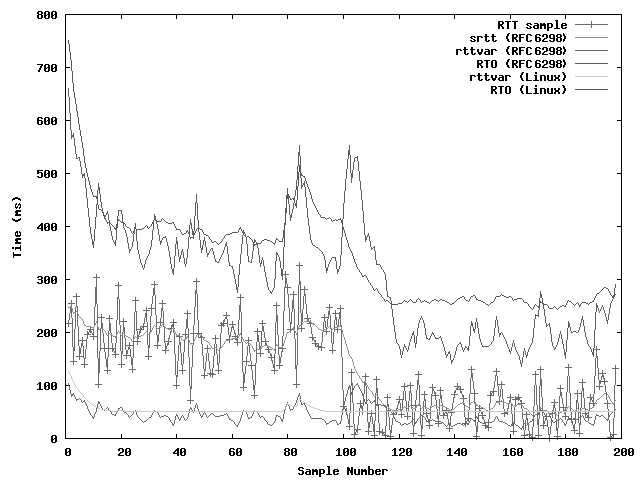
\includegraphics[width=0.7\textwidth]{imgs/14/14-3.png}
	\caption{对于200个伪随机的样本点采用 Linux 方法和标准方法来设置 RTO 和估算 RTT。前100个点是基于分布 N(200,50),后100个则基于N(50,50),且对负值进行了符号变换。Linux 将最小
    RTO设为200ms,而标准方法在样本120之后则变得更为密集。Linux 避免 RTO 设置过小就是防止这种情况的发生。标准方法在样本 78 和191 出现潜在问题}
\end{figure}

现在回到图 14-2,当接收端生成 ACK 7001时,我们看到其 TSER 包含了一个 TSV 副本,该值并非来自最新到达的报文段,而是最早的一个未经确认的报文段。当该ACK 返回
至发送端,通过计算得到的 RTT样本是基于第一个报文段,而非第二个。这说明了时间戳算法在延时或不稳定的ACK 下的工作情况。若计算最早的包对应的RTT,得到的样本值为
发送端期望收到 ACK 需经过的时间,而非实际网络 RTT。这点很重要,因为发送端需根据其ACK 接收率来设置 RTO,接收率可能小于包的发送率。

\subsection{RTT 估计器行为}
我们已经看到,设置 RTO 与估算 RTT有大量的设计和改进方法。图14-3显示了其中主要的估算方法,即基于标准方法和 Linux 算法得到的综合数据集。图中[RFC6298] 推荐的标
准算法最小 RTO 值1s 已被移除。目前的大多数 TCP 实现方法都不再采用该值[RKS07]。

图中显示了两个在高斯概率分布 N(200,50) 和 N(50,50)上的200个值对应的时间序列图。第一个分布对应前100个点,第二个对应后100个点。负的样本值通过符号变换转化为
正值(只针对第二个分布)。每个加号(+)表示一个具体的样本值。很明显可以看到,在第100个样本值之后出现了巨幅下降,另外 Linux 方法在第100个样本值之后 RTO 立即减小,
而标准方法则在120个样本值后才开始减小。

观察 Linux 的 rttvar线,可以看到其基本保持恒定。这是由于 \verb|mdev_max| 的最小值力50ms(因此 rtvar 也是如此),使得 Linux 的RTO 始终保持在200ms 以上,并且避免了所有
不必要的重传(尽管可能由于 RTO 较大,计时器未超时,导致丢包时性能降低)。标准方法在样本78和191 可能出现潜在问题,即伪重传的发生。这个问题留到后面再讨论。

\subsection{RTTM 对丟包和失序的鲁棒性}

当没有丢包情况时,不论接收端是否延迟发送ACK,TSOPT 可以很好地工作。该算法在以下几种情况下都能正确运行:
\begin{itemize}
    \item 失序报文段:当接收端收到失序报文段时,通常是由于在此之前出现了丢包,应当立即返回 ACK 以启动快速重传算法(见14.5节)。该ACK的TSER 部分包含的 TSV值为接收端收到最近的有序报文段的时刻(即最新的使窗口前进的报文段,通常不会是失序报文段)。这会使得发送端RTT样本增大,由此导致相应的RTO增大。这在一定程度上是有利的,即当包失序时,发送端有更多的时间去发现是出现了失序而非丢包,由此可避免不必要的重传。
    \item 成功重传:当收到接收端缓存中缺失的报文段时(如成功接收重传报文段),窗口通常会前移。此时对应 ACK 中的TSV 值来自最新到达的报文段,这是比较有利的。若采用原来报文段中的TSV,可能对应的是前一个 RTO,导致发送端 RTT 估算的偏离。
\end{itemize}

图14-4的例于描述了这些点。假设三个报文段,每个包含1024字节,接收顺序如下:报文段1包含1~1024字节,报文段3包含2049~3027字节,接着是报文段2包含1025~2048字节。

当报文段失序,返回的时间戳为最新的使窗口前移的报文段(而非到达接收端的最大的时间微)。这将使得发送端 RTO 在包失序期间过高估计 RTT,并降低其重传积极性

图14-4中发回的ACK 1025 包含了报文段1的时间戳(正常的数据确认),以及另一个包含报文段1时间戳的ACK 1025(对应于在窗口中但失序的重复 ACK),接着是 ACK 3037
包含了报文段2的时间戳(而非报文段3的时间戳)。当分组失序(或丢失)时,RTT会被过高估算。较大的 RTT 估计值使得 RTO也更大,由此发送端也不会急于重传。在失序情况下
这是很有利的,因为过分积极的重传可能导致伪重传。

我们已经看到,时间戳选项使得发送端即使在丢包、延时、失序的情况下也能测量RTT。发送端在测量 RTT 的过程中,可以在其选项中包含任意值,但其单位必须至少和实
际时间成比例,且粒度合理,并与TCP 序列号兼容,连接速率可信(详见[RFC1323])。特别是,为了对发送端更有利,对任何可信的 RTT,TCP 时钟必须至少“滴答”一次。另外,
其每次变化不能快于59ns。若小于,在IP 层允许单个包存在的最大时间(255s)内,记录TCP 时钟的32位的 TSV 值能够环绕[ID1323b]。满足上述所有条件后,RTO值就可以用来
触发重传。

\section{基于计时器的重传}
一旦 TCP发送端得到了基于时间变化的 RTT测量值,就能据此设置RTO,发送报文段时应确保重传计时器设置合理。在设定计时器前,需记录被计时的报文段序列号,若及时收
到了该报文段的ACK,那么计时器被取消。之后发送端发送一个新的数据包时,需设定一个新的计时器,并记录新的序列号。因此每一个 TCP 连接的发送端不断地设定和取消一个
重传计时器;如果没有数据丢失,则不会出现计时器超时。

\begin{tcolorbox}
    该过程对主机操作系统设计者来说可能难以理解。对典型的操作系统来说,计时器用于标记大量事件,计时器的实现也仅限于有效地设定和触发超时(需要调
    用系统函数)。然而对TCP 来说,计时器需要有效地实现被设置、重新设置或取消的功能;若TCP正常工作,则计时器不会出现超时的情况。
\end{tcolorbox}

若在连接设定的RTO 内,TCP没有收到被计时报文段的ACK,将会触发超时重传。我们已经在图14-1中看到这一过程。TCP 将超时重传视为相当重要的事件,当发生这种情况
时,它通过降低当前数据发送率来对此进行快速响应。实现它有两种方法:第一种方法是基于拥塞控制机制减小发送窗口大小(见第16章);另一种方法为每当一个重传报文段被再次
重传时,则增大RTO 的退避因子,即前面提到的Kar 算法的“第二部分”。特别是当同一报文段出现多次重传时,RTO 值(暂时性地)乘上值y来形成新的超时退避值:
\begin{equation}
RTO = yRTO
\end{equation}

在通常环境下,»值为1。随着多次重传,》呈加倍增长:2,4,8,等等。通常y不能超过最大退避因子(Linux 确保其 RTO 设置不能超过 \verb|TCP_RTO_MAX|,其默认值为120s)。
一旦接收到相应的ACK,》会重置为1。

\subsection{例子}

我们通过建立一个与图14-1 和图14-2相似的连接来观察重传计时器的行为。这里故意两次将序列号为 1401 的报文段丢弃(见图14-5)。

在本例中,我们可以利用一个特殊函数将某个序列号的报文段多次丢弃。这与图14-2相比,将会使 RTT引入一定的延时。连接建立之初与之前类似,仅当发送序列号为1和
1401 的报文段时,后一个包才被丢弃。当一个报文段到达接收端时,接收端并没有立即给出响应而是延迟发送ACK。在219ms 内都没有得到回应,发送端的计时器超时,导致序列号
为1的包被重传(此时的 TSV 值力577)。随即该包的到达使得接收端返回一个ACK。由于该 ACK 确认了数据被成功接收,并使得窗口前移,其TSER 值被用于更新 srtt 和 RTO 分别
为34 和234。

接着返回了三个 ACK,带星号(*)的ACK为重复ACK,但含了SACK 信息。我们将在14.5节和14.6节讨论重复ACK 和SACK。现在,由于这些ACK并没有使发送窗曰前移,
这些 TSER 值不会被采用。

随着最后一次重传以及报文段1401 到达(在TCP 时钟为911的时刻),修复阶段完成,接收端返回序列号为7001的ACK,表明所有数据已成功接收。

当网络无法正常传输数据时,重传计时器为 TCP 连接提供了“最后一招的重新启动”。在大多数情况下,计时器超时并触发重传是不必要的(也不是期望的),因为RTO的政路通
常大于 RTT(约2倍或更大),因此基于计时器的重传会导致网络利用率的下降。幸运的是,TCP 有另一种方法来检测和修复丢包,它比超时重传更为高效。由于它并不需要计时器超时
来触发,因此称为快速重传。

\section{快速重传}
快速重传机制[RFC5681]基于接收端的反馈信息来引发重传,而非重传计时器的超时。因此与超时重传相比,快速重传能更加及时有效地修复丢包情况。典型的TCP 同时实现了
两者。在详细讨论快速重传前,首先需要了解当接收到失序报文段时,TCP 需要立即生成确认信息(重复 ACK),并且失序情况表明在后续数据到达前出现了丢段,即接收端级存出现
了空觖。发送端的工作即为尽快地、高效地填补该空映。

当失序数据到达时,重复ACK应立即返回,不能延时发送。原因在于使发送端尽早得知有失序报文段,并告诉其空缺在哪。当采用SACK 时,重复ACK 通常也包含SACK 信
息,利用该信息可以获知多个空峡。

重复 ACK(不论是否包含SACK 信息)到达发送端表明先前发送的某个分组已丢失。在14.8节中我们会更详细地讨论到,重复 ACK 也可能在另一种情况下出现,即当网络中出现
失序分组时——若接收端收到当前期盼序列号的后续分组时,当前期盼的包可能丢失,也可能仅为延迟到达。通常我们无法得知是哪种情况,因此TCP 等待一定数目的重复ACK(称
为重复 ACK 网位或 dupthresh),来决定数据是否丢失并触发快速重传。通常,dupthresh 为常量(值为3),但一些非标准化的实现方法(包括Linux)可基于当前的失序程度动态调节
该值(见14.8节)。

快速重传算法可以概括如下:TCP 发送端在观测到至少 dupthresh 个重复ACK 后,即重传可能丢失的数据分组,而不必等到重传计时器超时。当然也可以同时发送新的数据。根据
重复 ACK 推断的丢包通常与网络拥塞有关,因此伴随快速重传应触发拥塞控制机制(详见第16章)。不采用SACK 时,在接收到有效ACK 前至多只能重传一个报文段。采用SACK,
ACK 可包含额外信息,使得发送端在每个 RTT 时间内可以填补多个空映。在描述一个基本快速重传算法的例子之后,我们将讨论快速重传中SACK 的用法。

\subsection{例子}
在下面的例子中,我们建立一个与图14-4类似的连接,但这次丢奔报文段23801 和26601,并且禁用SACK。我们将看到 TCP怎样利用基本的快速重传算法来填补空缺。发送
端为 Linux 2.6 系统,接收端为 FreeBSD 5.4 系统。图14-6可通过 Wireshark 的“统计ITCP流图| 时间序列图”(Statistics | TCP Stream Graph | Time-Sequence Graph)功能(toptrace)得
到,该图显示了快速重传行为。


\begin{figure}[!htb]
	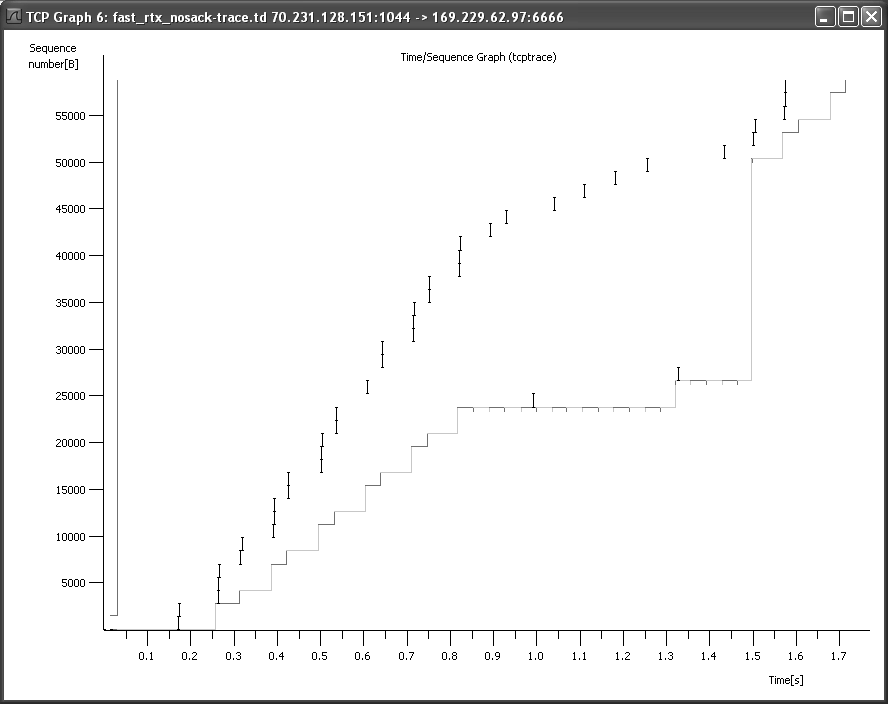
\includegraphics[width=1.0\textwidth]{imgs/14/14-6.png}
	\caption{本图中, 轴为TCP序列号,x轴为时间。发出的报文段用较深的黑色线段标出,收到的ACK 号用浅灰线。在0.993s到达的第三个重复 ACK 触发快速重传。该连接未采用SACK,所以每个 RTT 内至多只能填补一个空缺。
    之后到达的重复ACK 使得发送端发送新报文段(非重传报文段)。在1.32s 时刻到达的“部分ACK”再次触发了重传}
\end{figure}


该图y轴表示相对发送序列号,x轴表示时间。黑色的I形线段表示传输报文段的序列号范围。Wireshark 中的蓝色(图14-6中的浅灰色)线段为返回的ACK号。约1.0s时刻,序
列号 23801发生了快速重传(初始传输不可见,因为被发送端 TCP 下层丢弃)。第三个重复ACK 的到达触发了快速重传,图中表现为重叠的浅灰色线段。通过 Wireshark 的基本分析窗
口也可以观察到重传过程(见图14-7)。

图14-7的第一行(40号)为ACK 23801首次到达。Wireshark 标示出了(红色,在图14-7中看来是黑色)其他“有趣的”TCP 包。这些包与其他没有丢失或异常的包不同。我
们可以看到窗口更新、重复 ACK 和重传。0.853s时刻的窗口更新为带重复序列号的ACK(因为没有携带数据),但包含了 TCP 流控窗口的变动。窗口由231616字节变为233016字节。
因此,它并没有等到三个重复 ACK 来触发快速重传。窗口更新仅是提供了窗口通告的一个副本。我们将在第15 章中详细讨论。

0.8908、0.9268 以及 0.964s时刻到达的均为序列号为23801 的重复ACK。第三个重复ACK 的到达触发了报文段23801的快速重传,时间为0.993S。该过程也可通过 Witreshark 的
“统计|流图”(Statistics | Flow Graph)功能来观测(见图14-8)。

\begin{figure}[!htb]
	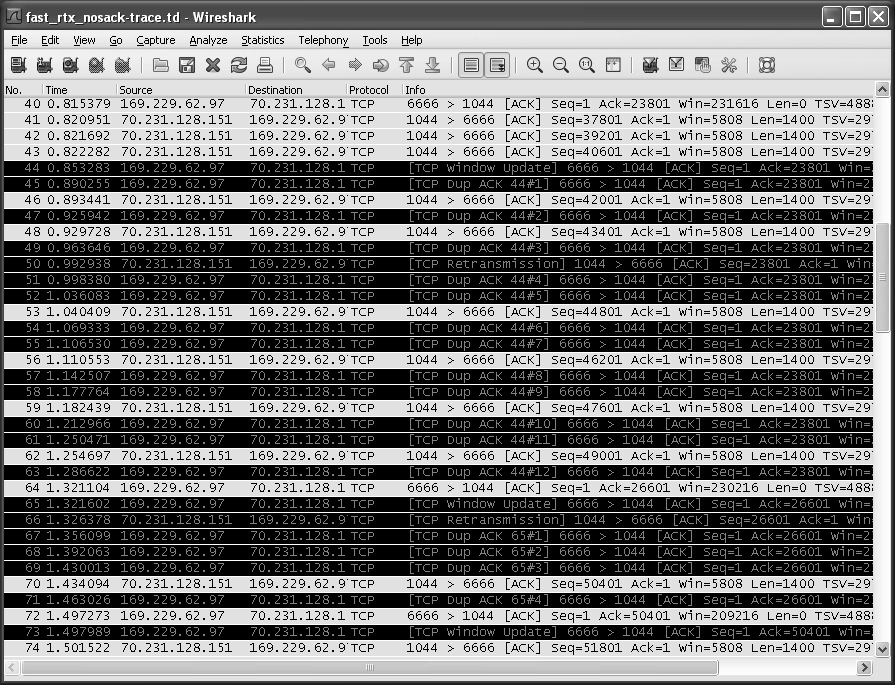
\includegraphics[width=1.0\textwidth]{imgs/14/14-7.png}
	\caption{TCP 交换的相对序列号。包50和66为重传。包50是由三次重复ACK 引发的快速重传。由于没有重传计时器超时,所以恢复过程相对较快}
\end{figure}

现在我们换个角度来看0.993s 时刻的快速重传过程,也可以看1.326s时刻发生的第二次快速重传,该重传是由1.322s时刻达到的ACK 触发的。

第二次重传与第一次有所不同。当第一次重传发生时,发送端在执行重传前已发送的最大序列号为(43401 +1400=44801),称恢复点(recovery point)。TCP 在接收到序列
号等于或大于恢复点的ACK 时,才会被认为从重传中恢复。本例中,1.322s 和1.321s时刻的ACK 并不是44801,而是26601。该序列号大于之前接收到的最大ACK 值(23801),但
不足以到达恢复点(44801)。因此这种类型的ACK 称为部分 ACK (partial ACK)。当部分ACK到达时,TCP 发送端立即发送可能丢失的报文段(这里是26601),并且维持这一过程
直到到达或超过恢复点。如果拥塞控制机制允许(见第16章),也可以同时发送新的数据。

这里的例子并没有采用SACK,不论是快速重传,还是基于“NewReno”算法[RFC3782] 恢复阶段执行的其他重传。由于没有SACK,通过观察返回的ACK 号的增长情
况,发送端在每个 RTT 内只能获知至多一个空缺。

在恢复阶段的具体行为根据 TCP发送端和接收端的类型和配置差异有所不同。这里描述的是无 SACK 发送端采用NewReno算法的例子,这种配置比较常见。根据NewReno算
法,部分ACK 只能使发送端继续处于恢复状态。对较旧的TCP 版本(单纯的Reno 算法)来说,没有部分ACK 这个概念,任何一个可接受的ACK(序列号大于之前接收到的所有
ACK)都能使发送端结束恢复阶段。这种方法可能会使 TCP 出现一些性能问题,我们在第16章会详细讨论。下面讨论 NewReno和SACK,它们有时也被称为“高级丢失恢复”技术,
以此来区别旧的方法。
\begin{figure}[!htb]
    \centering
	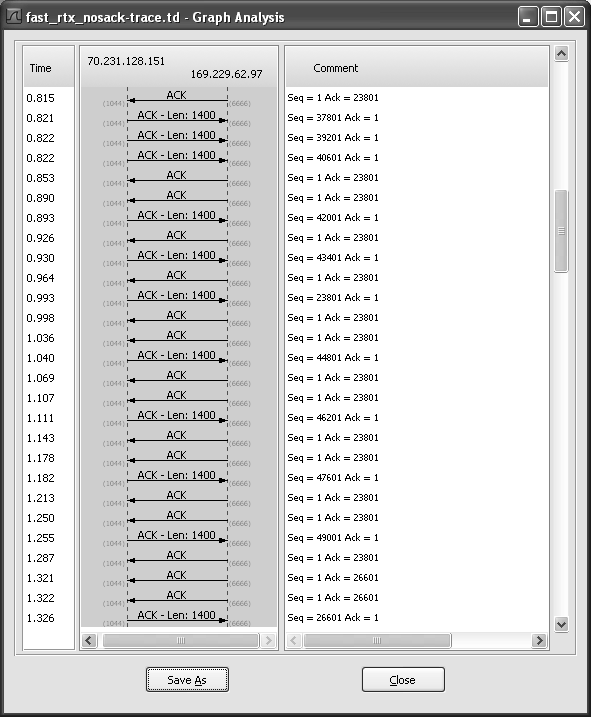
\includegraphics[width=0.5\textwidth]{imgs/14/14-8.png}
	\caption{0.890s、0.926s以及 0.964s 时刻到达的三次重复ACK 触发了0.993s 时刻的快速重传。0.853s时刻的ACK 并不算作重复ACK,因力它包含了一个窗口更新}
\end{figure}

\section{带选择确认的重传}

随着选择确认选项的标准化[RFC2018],TCP 接收端可提供SACK 功能,通过TCP头部的累积 ACK 号字段来描述其接收到的数据。之前提到过,ACK 号与接收端缓存中的其他
数据之间的间隔称为空缺。序列号高于空缺的数据称为失序数据,因为这些数据和之前接收的序列号不连续。

TCP发送端的任务是通过重传丢失的数据来填补接收端缓存中的空缺,但同时也要尽可能保证不重传已正确接收到的数据。在很多环境下,合理采用SACK 信息能更快地实现空缺
填补,且能减少不必要的重传,原因在于其在一个 RTT 内能获知多个空缺。当采用SACK选项时,一个 ACK 可包含三四个告知失序数据的SACK信息。每个 SACK 信息包含32位
的序列号,代表接收端存储的失序数据的起始至最后一个序列号(加1)。

SACK 选项指定n个块的长度为8n +2字节,因此40字节可包含最多4个块。通常SACK 会与TSOPT 一同使用,因此需要额外的10个字节(外加2字节的填充数据),这意味
着SACK 在每个 ACK 中只能包含3个块。

3个块表明可向发送端报告3个空缺。若不受拥塞控制(见第16章)限制,利用SACK选项可在一个 RTT 时间填补3个空映。包含一个或多个SACK块的ACK 有时也简单称为“SACK"。

\subsection{SACK 接收端行为}
接收端在 TCP 连接建立期间(见第13章)收到SACK许可选项即可生成SACK。通常来说,每当缓存中存在失序数据时,接收端就可生成SACK。导致数据失序的原因可能是由
于传输过程中丢失,也可能是新数据先于旧数据到达。这里只讨论第一种情况,后一种留待以后再讨论。

第一个 SACK 块内包含的是最近接收到的(most recently received) 报文段的序列号范围。由于SACK 选项的空间有限,应尽可能确保向TCP发送端提供最新信息。其余的
SACK 块包含的内容也按照接收的先后依次排列。也就是说,最新一个块中包含的内容除了包含最近接收的序列号信息,还需重复之前的SACK 块(在其他报文段中)。

在一个 SACK 选项中包含多个 SACK块,并且在多个 SACK 中重复这些块信息的目的在于,为防止SACK 丢失提供一些备份。若SACK 不会丢失,[RFC2018]指出每个 SACK
中包含一个SACK块即可实现 SACK 的全部功能。不幸的是,SACK 和普通的ACK 有时会丢失,并且若其中不包含数据(SYN或FIN 控制位字段不被置位)就不会被重传。

\subsection{SACK发送端行为}
尽管一个支持SACK 的接收端可通过生成合适的SACK 信息来充分利用SACK,但还不足以使该TCP 连接充分利用SACK 功能。在发送端也应提供SACK 功能,并且合理地利
用接收到的SACK 块来进行丢失重传,该过程也称为选择性重传(selective retransmission)或选择性重发(selective repeat)。SACK 发送端记录接收到的累积 ACK 信息(像大多数 TCP
发送端一样),还需记录接收到的SACK 信息,并利用该信息来避免重传正确接收的数据。一种方法是当接收到相应序列号范围的ACK 时,则在其重传缓存中标记该报文段的选择重传成功。

当SACK 发送端执行重传时,通常是由于其收到了 SACK 或重复ACK,它可以选择发送新数据或重传旧数据。SACK 信息提供接收端数据的序列号范围,因此发送端可据此推断
需要重传的空缺数据。最简单的方法是使发送端首先填补接收端的空缺,然后再继续发送新数据『RFC3517](若拥塞控制机制允许)。这也是最常用的方法。

该行为有一个例外。在[RFC2018] 中,SACK 选项和SACK块的当前规范是建议性的(advisory)。这意味着接收端可能提供一个 SACK 告诉发送端已成功接收一定序列号范围的
数据,而之后做出变更(“食言”)。由于这个原因,SACK 发送端不能在收到一个 SACK后立即清空其重传缓存中的数据;只有当接收端的普通TCP ACK 号大于其最大序列号值时才
可清除。这一规则同样影响重传计时器超时的行为。当TCP 发送端启动基于计时器的重传时,应忽略SACK 显示的任何关于接收端数据失序的信息。如果接收端仍存在失序数据,那
么重传报文段的ACK 中就包含附加的SACK 块,以便发送者使用。幸运的是,食言情况很少出现,也应尽量避免出现。

\subsection{例子}
为理解SACK怎样影响发送端和接收端的行为,我们重复前面的快速重传实验,参数设置也如前(丢掉序列号 23601 与28801),但这次发送端和接收端都采用SACK。为准确观测
到实验过程,我们仍采用 Wireshark 的 TCP 序列号(tcptrace)图功能(见图14-9)。
\begin{figure}[!htb]
    \centering
	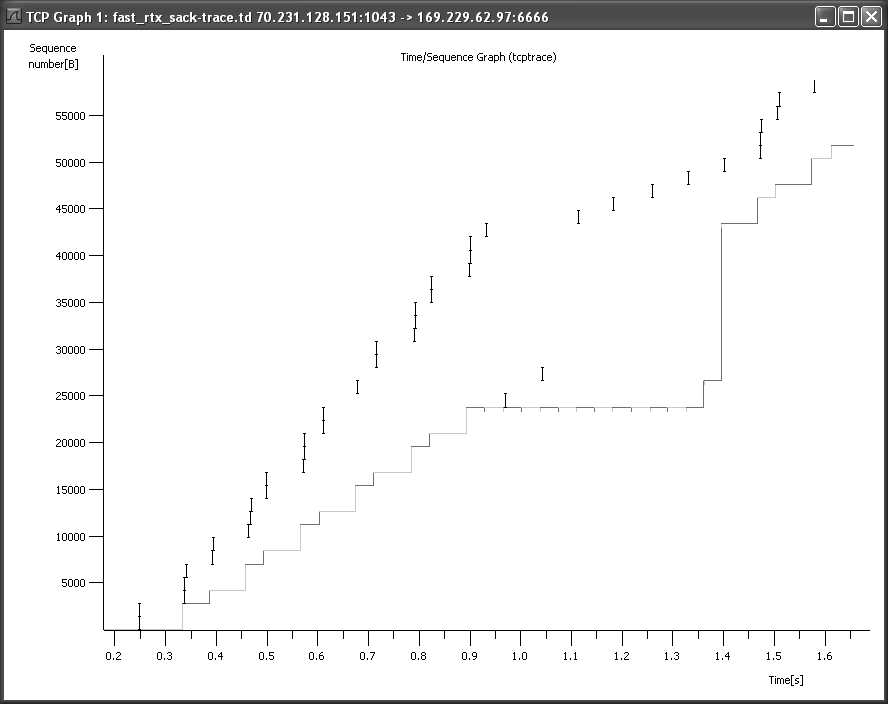
\includegraphics[width=0.7\textwidth]{imgs/14/14-9.png}
	\caption{第一个包含SACK 信息的重复ACK 触发了快速重传。后一个ACK 的到达使得发送端了解到第二个丢失的报文段,并在同一个 RTT 内重传了该报文段}
\end{figure}

图14-9与图14-6类似,但利用SACK信息,发送端在重传完报文段23601 后,不必等待一个 RTT 再重传丢失报文段28801。后面将仔细讨论这些内容,现在我们首先在连接建立
过程中验证 SACK 允许(SACK-Permitted) 选项的存在,见图14-10。

\begin{figure}[!htb]
    \centering
	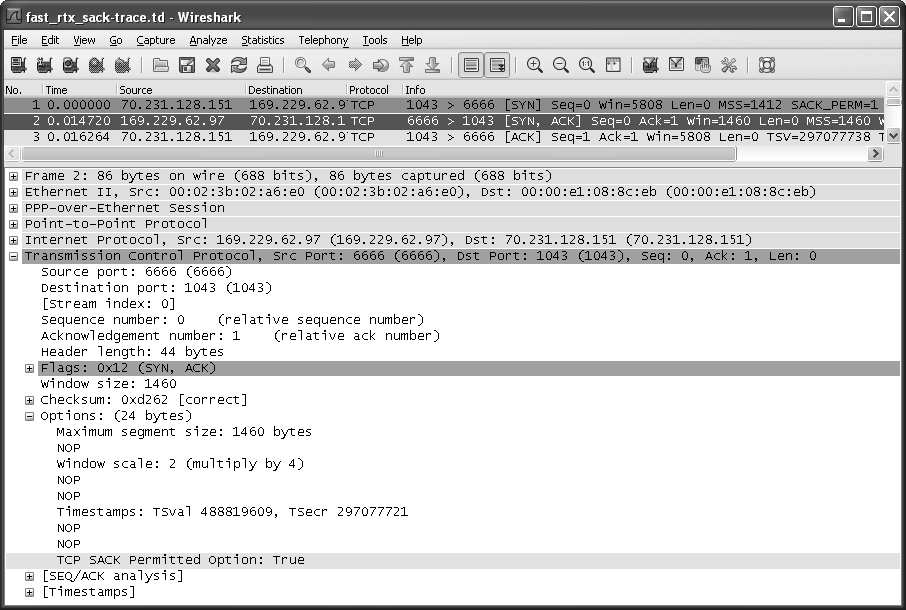
\includegraphics[width=0.9\textwidth]{imgs/14/14-10.png}
	\caption{SYN 报文段中SACK 允许选项表明可生成和发送SACK信息。现在的大部分 TCP 版本在连接建立阶段都支持 MSS,时间戳,窗口扩大以及 SACK 允许选项}
\end{figure}

与预计的一样,接收端通过SACK允许选项来使用SACK。发送端的SYN 包,即记录的第一个包,也包含了该选项。这些选项只在连接建立阶段才能看到,因此只出现在SYN置位的报文段中。

一旦连接被允许使用SACK,发生丢包即会使得接收端开始生成SACK。Wireshark 显示了第一个 SACK 选项的内容(见图14-11)。

\begin{figure}[!htb]
    \centering
	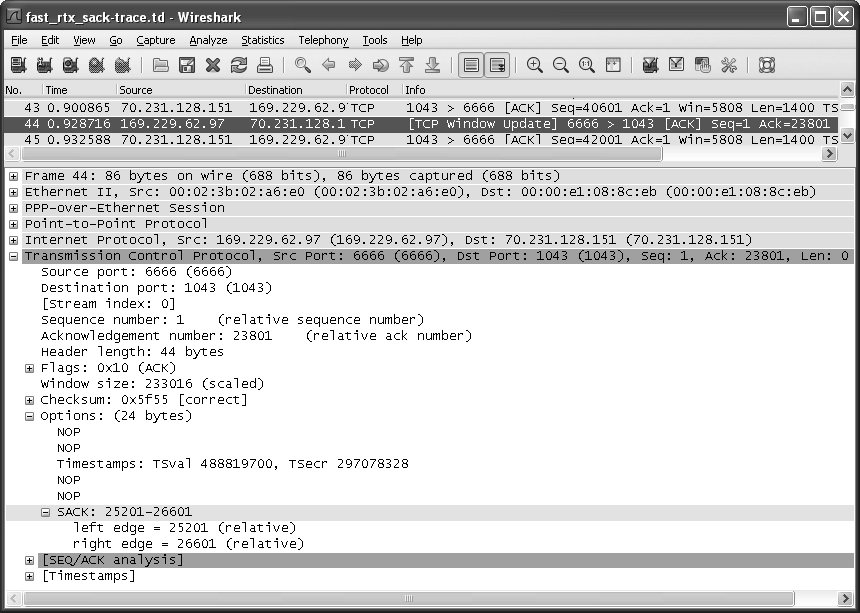
\includegraphics[width=0.7\textwidth]{imgs/14/14-11.png}
	\caption{第一个 ACK 包含SACK 信息表明失序数据的序列号范围为 25201 至 26601}
\end{figure}

图14-11 显示了首个SACK 被接收后的一系列事件。Wireshark 通过SACK 范围的左右边界来表示 SACK 信息。这里我们看到 23801的ACK 包含了一个SACK 块[25201,26601],
指明接收端的空缺。接收端敏失的序列号范围为[23801,25200],相当于一个从序列号23801开始的 1400字节的包。注意到该 SACK 为一次窗口更新,并不能算作重复ACK,之
前也提到过,因此不能触发快速重传。

0.967S时刻到达的SACK 包含两个块:[28001,29401]和[25201, 26601]。回忆一下前面提过的,为提高对 ACK 丢失的鲁棒性,前面SACK 的第一个块需要重复出现在后续
SACK 的靠后的位置。该SACK 为序列号23801的重复 ACK,表明接收端现在需要从序列号23801至26601 的两个全长报文段。发送端立即响应,启动快速重传,但由于拥塞控制机
制(见第16章),发送端只重传了一个报文段23801。随着另外的两个ACK 的到达,发送端被允许发送第二个重传报文段26601。

TCP SACK 发送端借鉴了 NewReno算法中的恢复点的思想。本例中,在重传前发送的最大序列号为 43400,低于图14-5所示的NewReno算法的例子。这里的SACK 快速重传实
现中,不需要三次重复 ACK;TCP 更早地启动了重传,但恢复的出口本质上是一致的。一且接收到序列号 43401 的 ACK,即1.3958s时刻,恢复阶段即完成。

值得注意的是,发送端采用SACK 并不能百分百地提高整体传输性能。我们来看之前讨论过的这两个例子,NewReno 发送端(非 SACK)完成131 074字节的数据传输用时3.529s,
而SACK 发送端则用了3.674s。尽管这两个值不能这样直接比较,因为两者所处的网络环境并非绝对相同(这不是仿真实验,而是在真实环境中的测试),但极为近似。在RTT较大,
丢包严重的情况下,SACK 的优势就能很好地体现出来,因为在这样的环境下,一个 RTT内能填补多个空缺显得尤为重要。

\section{伪超时与重传}
在很多情况下,即使没有出现数据丢失也可能引发重传。这种不必要的重传称为伪重传 (spurious retransmission),其主要造成原因是伪超时(spurious timeout),即过早判定超时,
其他因素如包失序、包重复,或ACK 丢失也可能导致该现象。在实际 RTT 显著增长,超过当前 RTO 时,可能出现伪超时。在下层协议性能变化较大的环境中(如无线环境),这种情
况出现得比较多,[KP87]中也提到。这里我们仅关注由伪超时导致的伪重传。失序与重复的影响在下面的章节中再讨论。

为处理伪超时问题提出了许多方法。这些方法通常包含检测(detection)算法与响应(response)算法。检测算法用于判断某个超时或基于计时器的重传是否真实,一旦认定出现
伪超时则执行响应算法,用于撤销或减轻该超时带来的影响。本章中我们只讨论报文段重传行为。典型的响应算法也涉及拥塞控制变化,会在第16章讨论。

图14-12描述了一个简化的TCP 交换过程。在报文段8发送完成后 ACK 链路上出现了延迟高峰导致了一次伪重传。在报文段5超时重传后,原始传输的报文段5~8的ACK
仍然处于在传状态。本图中为简便起见,序列号和 ACK号都基于包而非字节来表示,并且ACK 号表示已接收到的包,而非期望接收的下一个包。当这些 ACK 到达时,发送端继续重
传早已接收的其他报文段,从已确认的报文段之后开始。这导致 TCP 出现了“回退 N”(g0-back-N)的行为模式,并产生了更多的重复 ACK 返回发送端,这时就可能会触发快速重传。
针对这一问题,提出了一些方法来减轻不良影响。下面我们讨论其中比较常用的几种方法。

\subsection{重复 SACK (DSACK)扩展}
在非SACK 的TCP 中,ACK 只能向发送端告知最大的有序报文段。采用SACK 则可告知其他的(失序)报文段。基本的SACK 机制对接收端收到重复数据段时怎样运作没有规定。
这些重复数据可能是伪重传、网络中的重复或其他原因造成的。

在传输完报文段8后出现了一次延迟高峰,导致了报文段5的伪超时和重传。重传完成后,首次传输的报文段5对应的ACK 到达。报文段5的重传使得接收端收到了重复报文段,紧接着又重传了报文段6、7、8,尽管在接收端已存在这些报文段,整个连接还是执行了“回退N”行为

在SACK 接收端采用 DSACK(或称作 D-SACK),即重复 SACK[RFC2883],并结合通常的 SACK 发送端,可在第一个 SACK 块中告知接收端收到的重复报文段序列号。DSACK
的主要目的是判断何时的重传是不必要的,并了解网络中的其他事项。因此发送端至少可以推断是否发生了包失序、ACK 丢失、包重复或伪重传。

DSACK 相比于传统SACK 并不需要额外的协商过程。为使其正常工作,接收端返回的SACK 的内容会有所改变,对应的发送端的响应也会随之变化。如果一个非 DSACK 与
DSACK 的 TCP 共用一个连接,它们会交互操作,但非DSACK 不能使用DSACK 的功能。

SACK 接收端的变化在于,允许包含序列号小于(或等于)累积 ACK 号字段的SACK块。这并非SACK 的本意,但这样做能很好地配合该目的。(在 DSACK 信息高于累积 ACK
号字段的情况下,即出现重复的失序报文段时,它也能很好地工作。)DSACK 信息只包含在单个 ACK 中,该ACK 称为DSACK。与通常的SACK 信息不同,DSACK 信息不会在多个
SACK 中重复。因此,DSACK 较通常的 SACK 鲁棒性低。

[RFC2883]没有具体规定发送端对DSACK 怎样处理。[RFC3708] 给出了一种实验算法,利用DSACK来检测伪重传,但它并没有提供响应算法。它提到可采用 Eifel 响应算法,我
们在14.7.4 节中会讨论,在此之前我们先介绍一些其他的检测算法。

\subsection{Eifel 检测算法}
本章开头,我们讨论了重传二义性问题。实验性的 Eifel 检测算法TRFC3522]利用了TCP的ISOPT来检测伪重传。在发生超时重传后,Eifel 算法等待接收下一个ACK,若为针
对第一次传输(即原始传输)的确认,则判定该重传是伪重传。

利用Eifel 检测算法能比仅来用DSACK 更早检测到伪重传行为,因为它判断伪重传的ACK 是在启动丢失恢复之前生成的。相反,DSACK 只有在重复报文段到达接收端后才能发
送,并且在DSACK返回至发送端后才能有所响应。及早检测伪重传更为有利,它能使发送端有效避免前面提到的“回退N”行为。

Eifel 检测算法的机制很简单。它需要使用TCP 的TSOPT。当发送一个重传(不论是基于计时器的重传还是快速重传)后,保存其 TSV 值。当接收到相应分组的ACK 后,检查该
ACK 的TSER 部分。若 TSER值小于之前存储的TSV 值,则可判定该ACK 对应的是原始传输分组,即该重传是伪重传。这种方法针对ACK 丢失也有很好的鲁棒性。如果一个ACK
丢失,后续ACK 的TSBR 值仍比存储的重传分组的TSV小。该窗口内的任一ACK 的到达都能判断是否出现伪重传,因此单个ACK 的丢失不会造成太大问题。

Eifel 检测算法可与DSACK 结合使用,这样可以解决整个窗口的ACK 信息均丢失,但原始传输和重传分组都成功到达接收端的情况。在这种特殊情况下,重传分组的到达会生成
一个 DSACK。Eifel 算法会理所当然地认定出现了伪重传。然而,在出现了如此之多的ACK丢失的情况下,使得 TCP 相信该重传不是伪重传是有用的(例如,使其减慢发送速率—采
用拥塞控制的后果,第16章会讨论)。因此,DSACK 的到达会使得 Eifel 算法认定相应的重传不是伪重传。

\subsection{前移 RTO 恢复(F-RTO)}
前移 RTO 恢复(Forward-RTO Recovery,F-RTO)[RFC5682]是检测伪重传的标准算法。它不需要任何 TCP选项,因此只要在发送端实现该方法后,即使针对不支持 TSOPT 的接收
端也能有效地工作。该算法只检测由重传计时器超时引发的伪重传;对之前提到的其他原因引起的伪重传则无法判断。

在一次基于计时器的重传之后,F-RTO 会对TCP的常用行为做出一定修改。由于这类重传针对的是没有收到 ACK 信息的最小序列号,通常情况下,TCP 会继续按序发送相邻的
分组,这就是前面描述的“回退N”行为。

F-RTO 会修改 TCP 的行 ,在超时重传后收到第一个 ACK 时,TCP 会发送新(非重传)数据,之后再响应后一个到达的ACK。如果其中有一个为重复ACK,则认为此次重传没问
题。如果这两个都不是重复ACK,则表示该重传是伪重传。这种方法比较直观。如果新数据的传输得到了相应的ACK,就使得接收端窗口前移。如果新数据的发送导致了重复ACK,
那么接收端至少有一个或更多的空缺。这两种情况下,接收新数据都不会影响整体数据的传输性能(假设接收端有足够的存储空间)。

\subsection{Eifel 响应算法}
一旦判断出现伪重传,则会引发一套标准操作,即 Eifel 响应算法[RFC4015]。由于响应算法逻辑上与 Eifel 检测算法分离,所以它可与我们前面讨论的任一种检测方法结合使
用。原则上超时重传和快速重传都可使用Eifel 响应算法,但目前只针对超时重传做了相关规定。

尽管 Eifel 响应算法可结合其他检测算法使用,但根据是否能尽早(如 Eifel 检测算法或F-RTO)或较迟(如DSACK)检测出伪超时的不同而有所区别。前者称为伪超时,通过检查
ACK 或原始传输来实现。后者称为迟伪超时(late spurious timeout),基于由(伪)超时而引发的重传所返回的ACK 来判定。

响应算法只针对第一种重传事件。若在恢复阶段完成之前再次发生超时,则不会执行响应算法。在重传计时器超时后,它会查看 srt 和 rttvar 的值,并按如下方式记录新的变量
\verb|srtt_prev| 和 \verb|rttvar_prev|:

\begin{verbatim}
    srtt_prev = srtt + 2(G)
rttvar prev = rttvar
\end{verbatim}

在任何一次计时器超时后,都会指定这两个变量,但只有在判定出现伪超时才会使用它们,用于设定新的 RTO。在上式中,G代表TCP 时钟粒度。\verb|srtt_prev| 设为 sttt加上两倍的时钟
粒度是由于:srt的值过小,可能会出现伪超时。如果 srtt稍大,就可能不会发生超时。sttt加上2G 得到 \verb|srtt_prev|,之后都使用 \verb|srtt_prev| 来设置 RTO。

完成 \verb|srtt_prey| 和 \verb|rttvar_prev| 的存储后,就要触发某种检测算法。运行检测算法后可得到一个特殊的值,称为伪恢复(SpuriousRecovery)。如果检测到一次伪超时,则将伪恢复置为
\verb|SPUR_TO|。如果检测到迟伪超时,则将其置为 \verb|LATB_SPUR_TO|。否则,该次超时为正常超时,TCP继续执行正常的响应行为。

若伪恢复为 \verb|SPUR_TO.TCP|可在恢复阶段完成之前进行操作。通过将下一个要发送报文段(称为 SND.NXT)的序列号修改为最新的未发送过的报文段(称为 SND.MAX)。这样
就可在首次重传后避免不必要的“回退N”行为。如果检测到一次迟伪超时,此时已生成对首次重传的ACK,则SND.NXT 不改变。在以上两种情况中,都要重新设置拥塞控制状态
(见第16章)。并且一旦接收到重传计时器超时后发送的报文段的ACK,就要按如下方式更新 srtt、rttvar 和 RTO 的值:

这里,m是一个 RTT样本值,它是基于超时后首个发送数据收到的ACK 而计算得到的。进行这些变量更新的目的在于,实际的RTT值可能发生了很大变化,RTT 的当前估计值已
经不适合用于设置 RTO。若路径上的实际 RTT 突然增大(例如由于无线切换至一个新的基站),当前的 srtt和rttvar 就显得过小,应重新设置。而另一方面,RTT 的增大可能只是暂时
的,这时重设 srtt 和 rttvar 的值就不那么明智了,因为它们原先的值可能更为精确。

在新RTT 样本值较大的情况下,上述等式尽力获得上述两种情况的平衡。这样做可以有效地抛弃之前的 RTT 历史值(和 RTT 的历史变化情况)。只有在响应算法中 srtt和 rttvar
的值才会增大。若RTT 不会增大,则维持估计值不变,这本质上是忽略超时情况的发生。两种情况中,RTO还是按正常方式进行更新,并针对此次超时设置新的重传计时器值。

\section{包失序与包重复}
前面讨论的都是 TCP 如何处理包丢失的问题。这是普遍讨论的问题,而且针对包丢失的鲁棒性问题已经做了很多工作。在最后一个章节中可以看到,其他的包传输异常现象,如
重复和失序问题也会影响 TCP操作。在这两种情况中,我们希望 TCP 能区分是出现了失序或重复还是丢失。我们接下来会看到,正确区分这些情况并非易事。


\subsection{}
在IP网络中出现包失序的原因在于IP 层不能保证包传输是有序进行的。这一方面是有利的(至少对IP 层来说),因为IP 可以选择另一条传输链路(例如传输速度更快的路径),而
不用担心新发送的分组会先于旧数据到达,这就导致数据的接收顺序与发送顺序不一致。还有其他的原因也会导致包失序。例如,在硬件方面一些高性能路由器会采用多个并行数据链
路[BPS99],不同的处理延时也会导致包的离开顺序与到达顺序不匹配。

失序问题可能存在于 TCP 连接的正向或反向链路中(也可能两者同时存在)。数据段的失序与 ACK 包的失序对 TCP 的影响有一定差别。回忆一下,由于非对称路由,经常会出现
ACK 经不同于数据包的链路(和不同路由器)传输。

当传输出现失序时,TCP 可能会在某些方面受影响。如果失序发生在反向(ACK)链路,就会使得 TCP 发送端窗口快速前移,接着又可能收到一些显然重复而应被丢弃的ACK。由
于TCP 的拥塞控制行为(见第16章),这种情况会导致发送端出现不必要的流量突发(即瞬时的高速发送)行为,影响可用网络带宽。

如果失序发生在正向链路,TCP 可能无法正确识别失序和丢包。数据的丢失和失序都会导致接收端收到无序的包,造成数据之间的空缺。当失序程度不是很大(如两个相邻的包交
换顺序),这种情况可以迅速得到处理。反之,当出现严重失序时,TCP 会误认为数据已经丢失。这就会导致伪重传,主要来自快速重传算法。

回忆一下之前的讨论,快速重传是根据收到重复ACK 来推断出现丢包并启动重传,而不必等待重传计时器超时。由于 TCP 接收端会对接收到的失序数据立即返回ACK,以此来
帮助触发快速重传,因此网络中任何一个失序的数据包都会生成重复 ACK。由于网络中少量失序情况是常见的,假设一旦收到重复 ACK,发送端即启动快速重传,那么就会导致大量不
必要的重传发生。为解决这一问题,快速重传仅在达到重复阈值(dupthresh) 后才会被触发。

图14-13描述了上述情况。图中左半部分表示在轻微失序的情况下 TCP 的操作,这里的dupthresh 设为3。单个重复ACK 不会影响TCP的行。右半部分表示出现严重失序时的情
况。由于出现了3次失序,对应生成了3次重复 ACK,因此触发了快速重传,使得接收端收到了一个重复报文段。


轻徽失序(左)中,可忽略少量的重复ACK。当失序状况较为严重(右)时,这里4个包中有三个出现失序,就会触发伪快速重传

区分丢包与失序不是一个很重要的问题。要解决它需要判断发送端是否已经等待了足够长的时间来填补接收端的空缺。幸运的是,互联网中严重的失序并不常见[J03],因此将
dupthresh 设为相对较小值(如峡省值为3)就能处理绝大部分情况。即便如此,还是有很多研究致力于调整 TCP 行为来应对严重失序[LLY07]。有些方法可动态调整 dupthresh,如
Linux 的TCP实现。

\subsection{重复}
尽管出现得比较少,但IP协议也可能出现将单个包传输多次的情况。例如,当链路层
网络协议执行一次重传,并生成同一个包的两个副本。当重复生成时,TCP 可能出现混淆。考虑图14-14 中的情况,包3重复生成三个副本。

从图中可看到,包3的多次重复会使得接收端生成一系列的重复ACK,这足以触发伪快速重传,使得非 SACK
发送端误认为包5与包6更早到达。利用SACK(特别是DSACK),就可以简单地忽略这个问题。采用DSACK,每个A3的重复 ACK 都包含报文段3已成功接收的信息,并且没
有包含失序数据信息,意味着到达的包(或ACK)一定是重复数据。TCP 通常都可防止此类伪重传。

\section{目的度量}
从前面的讨论中我们看到,TCP 能不断“学习”发送端与接收端之间的链路特征。学习的结果显示为发送端记录一些状态变量,如srtt和 rttvar。一些 TCP 实现也记录一段时间内已出现的失序包的估计值。
一般来说,一旦该连接关闭,这些学习结果也会丢失,即与同一个接收端建立一个新的TCP连接后,它必须从头开始获得状态变量值。

较新的TCP 实现维护了这些度量值,即使在连接断开后,也能保存之前存在的路由或转发表项,或其他的一些系统数据结构。当创立一个新的连接时,首先查看数据结构中是否
存在与该目的端的先前通信信息。如果存在,则选择较近的信息,据此为 srtt、rttvar 以及其他变量设初值。在TCP 连接关闭前,可更新统计数据,通过替换现存数据或其他方式的
更新来实现。在Linux 2.6中,变量值更新为现存值中的最大值和最近测量的数据。可通过iproute2[IPR2]的相关工具来查看这些变量值:

\begin{verbatim}
    Linux& ip route show cache 132.239.50.184
132.239.50.184 from 10.0.0.9 tos 0x10 via 10.0.0.1 dev
mtu 1500 rtt 29ms rttvar 29ms cwnd 2 advmss 1460 hoplimit 64
\end{verbatim}


该命令利用特的DSCP 值(16,表示CS2,但值为 Ox10代表采用较旧日的“Tos”)显示了之前连接存储的信息,本地系统和 132.239.50.184之间采用IPv4,下一跳为10.0.0.1
网络设备为 ehto。我们可以看到包大小信息(由 PMTUD 得到路径MTU,由远端告知MSS)、最大跳步数(针对IPv6,这里没有用到)、stt 和 rttvar 的值,以及第16章中会讨论
的拥塞控制信息如 cwnd。

\section{重新组包}

当TCP超时重传,它并不需要完全重传相同的报文段。TCP允许执行重新组包(repacketization),发送一个更大的报文段来提高性能。(通常该更大的报文段不能超过接收
端通告的 MSS,也不能大于路径 MTU。)允许这样做的原因在于,TCP是通过字节号来识别发送和接收的数据,而非报文段(或包)号。

TCP能重传一个与原报文段不同大小的报文段,这从一定意义上解决了重传二义性问题。STODER[T2205] 就是基于该思想,采用重新组包的方法来检测伪超时。

我们可以很容易地观察到重新组包的过程。我们采用 sock 程序作为服务器,并用 Telnet连接它。首次我们输人一行信息 “hello there”。这就生成了一个13字节的数据段,包括回
车换行在内。接着断开网络连接,输人 “line number 2”(14字节,包括换行)。然后在等待约45秒后,输入“and 3",之后关闭连接:

在分析结果中,省略了初始SYN交换过程。前两个报文段包含数据字符串“hellothere ”及其确认信息。紧接着的包并非有序:它从序列号29开始,包含字符串 “and 3"(7
个字节)。它返回的ACK包含ACK 号14,但SACK 块的相对序列号为(29,36}。中间的数据已丢失。TCP 采用一个更大的包来重传,包含序列号14 ~36。因此,我们可以看到序
列号14数据的重传导致了一次重新组包,形成了 22 字节的较大包来传输。有趣的是,包中重复包含了 SACK 块中的数据,同时也将 FIN 位字段置位,表明这是连接关闭前最后传输的
数据。

\section{与TCP 重传相关的攻击}
有一类DoS 攻击称为低速率 DoS 攻击[KK03]。在这类攻击中,攻击者向网关或主机发送大量数据,使得受害系统持续处于重传超时的状态。由于攻击者可预知受害 TCP 何时
启动重传,并在每次重传时生成并发送大量数据。因此,受害 TCP 总能感知到拥塞的存在,根据 Kam 算法不断减小发送速率并退避发送,导致无法正常使用网络带宽。针对此类攻击
的预防方法是随机选择 RTO,使得攻击者无法预知确切的重传时间。

与 Dos相关但不同的一种攻击为减慢受害 TCP的发送,使得 RTT估计值过大。这样受害者在丢包后不会立即重传。相反的攻击也是有可能的:攻击者在数据发送完成但还未到达
接收端时伪造 ACK。这样攻击者就能使受害 TCP 认为连接的 RTT 远小于实际值,导致过分发送,造成大量的无效传输。


\section{总结}
本章详细讨论了 TCP 超时和重传策略。第一个例子描述了当TCP需要发送一个数据包时,简单地暂时断开网络,导致重传计时器超时触发了一次超时重传。每个后续重传与前一
次传输都间隔两倍时长,形成二进制指数退避,即 Kar 算法的第二部分。

TCP 测量 RTT 并用这些测量值记录平滑的RTT 与均值偏差估计值,用这两个估计值计算新的重传超时值。在不采用时间戳选项的情况下,TCP 在每个数据窗口只能测量一个
RTT。Kam 算法通过不测量重传报文段的 RTT样本值来避免重传二义性问题。现在的大部分TCP 版本都使用时间戳选项,使得每个报文段都能单独测量。时间戳选项即使在包失序
或包重复的情况下也能很好地工作。

我们还讨论了快速重传算法,它在计时器没有超时的情况下就能被触发。该算法可有效地(并最常用)填补由丢包引起的空缺。结合选择确认可更好地提高算法性能。选择确认在
ACK 中携带其他的信息,允许发送端在每个 RTT 内修补多个空觖,在某些环境下可有效提高传输性能。

如果 RTT 测量值小于连接的实际值,就可能发生伪重传。在这种情况下,若TCP 的等待时间稍长,(不必要的)重传就可能不会发生。针对伪超时问题提出了很多算法。DSACK
需要等到接收到重复报文段的ACK。Eifel 检测方法依据 TCP 时间戳,但它的响应速度能比DSACK 更快,这是因为它是根据超时前所发送报文段返回的ACK 来检测伪超时的。F-RTO
与 Eifel 算法类似,但不需要时间戳。它使得发送端在判断出现伪超时后发送新数据。以上这些检测算法都需要结合使用响应算法,我们讨论到的响应算法主要是 Eifel 响应算法。它
在延迟大幅增长的情况下(否则对超时不做任何响应),会重新设置 RTT 和 RTT变化估计值。

我们也讨论了 TCP 怎样存储连接状态,怎样重新组包,以及相关攻击,包括使得 TCP过分被动或过分积极。在第16章讨论 TCP拥塞控制时,我们会看到更多的此类攻击及其造
成的影响。
